% Created 2022-11-23 mer. 19:10
% Intended LaTeX compiler: pdflatex
\documentclass[a4paper]{article}
\usepackage[utf8]{inputenc}
\usepackage[T1]{fontenc}
\usepackage{graphicx}
\usepackage{longtable}
\usepackage{wrapfig}
\usepackage{rotating}
\usepackage[normalem]{ulem}
\usepackage{amsmath}
\usepackage{amssymb}
\usepackage{capt-of}
\usepackage{hyperref}
\author{Samuel Michaël Vanié}
\date{17th November 2022}
\title{Rapport Aod}
\hypersetup{
 pdfauthor={Samuel Michaël Vanié},
 pdftitle={Rapport Aod},
 pdfkeywords={},
 pdfsubject={},
 pdfcreator={Emacs 28.2 (Org mode 9.6)}, 
 pdflang={English}}
\begin{document}

\maketitle
\tableofcontents

\clearpage

\section{Introduction}
\label{sec:orgf2f739d}

Ce rapport relate ma compréhension des notions que j'ai appris tout au long du cours d'Algorithmique et Optimisation Discrète.

Pour commencer quel était l'objectif que j'ai pu ressentir au travers de ce cours ?
Pour moi l'objectif de ce cours était de me faire prendre conscience des mécanismes qui interviennent au niveau de la mémoire pendant l'exécution d'un programme mais aussi de me montrer certaines techniques permettant d'optimiser cette gestion des différents niveaux de mémoire.

Pour résumer, l'ordinateur a une hiérarchie de mémoires. Les mémoires vont des plus rapides et moins capacitives, plus proche du processeur aux mémoires avec plus de capacité mais beaucoup moins rapides.

Les mémoires ont une taille totale bien spécifique et une taille de ligne de cache qui représente l'unité de chargement des données. C'est à dire que pour charger les données en mémoire, l'ordinateur ne le fait par octet par octet ou bit par bit mais par taille de ligne de cache. Le passage d'un niveau du cache à un autre se fait aussi par ligne de cache.

Pour continuer, lors de l'exécution d'un programme, plusieurs manipulation sont effectuées au niveau des différentes mémoires : des \textbf{lectures} et des \textbf{chargements}. Les données passent aussi d'un niveau à un autre en fonction de la taille.

Lorsqu'un programme veut récupérer une donnée dans la mémoire il recherche dans le cache. Si la donnée se trouve dans le cache (\textbf{cache hit}), la donnée est chargé dans l'espace de travail et utilisé par le programme. Si la donnée est absente du cache (\textbf{cache miss} ou \textbf{défaut de cache}), la donnée ainsi que celles adjacentes sont chargées dans le cache dans l'espoir que celles-ci soient aussi accédées très prochainement.

Concernant les défauts de cache, ils peuvent intervenir au début de l'exécution d'un code, ces défauts la sont inévitables et sont appelés les \textbf{défauts de cache obligatoires}.
Lorsque le cache est plein alors qu'on doit y ajouter une nouvelle ligne, une ligne de cache déjà présente doit être remplacée. Pour effectuer cette opération plusieurs algorithmes existent. On appelle ces algorithmes les \textbf{politiques de remplacement}. Il en existe plusieurs tels que le \textbf{LRU} (\textbf{Last Recently Used}) que nous avons vu dans ce cours, le \textbf{FIFO} (First In First Out), le \textbf{LIFO} (Last In First Out) ou le \textbf{MRU} (\textbf{Most Recently Used}).


\section{Localité}
\label{sec:orgcbcfea2}


Pour amortir le coup d'un programme et le rendre plus efficace, il faudrait diminuer le nombre de défauts de cache que celui-ci fait. Ainsi pour y parvenir, nous devons soit accéder aux données qui sont stockées de manière contigüe dans la mémoire (\textbf{localité spatiale}) ou faire en sorte que les accès à une même donnée se fassent simultanément ou pendant une période de temps qui est très rapprochée (\textbf{localité temporelle}).

Dans la suite, j'utilise le LRU comme politique de remplacement ainsi que le modèle CO qui est un modèle théorique du cache utilisé pour faire les estimations sur le coup des opérations.


Pour illustrer les concepts de localité, comparons ces deux algorithmes.

\emph{Premier algorithme}

\begin{verbatim}
int somme = 0;
int somme_carres=0;
for(int i=0; i<sizeof(tab)/sizeof(int); i++){
    somme += tab[i];
}

for(int i=0; i<sizeof(tab)/sizeof(int); i++){
    somme_carres += pow(tab[i], 2);
}
\end{verbatim}

\emph{Deuxième algorithme}

\begin{verbatim}
int somme = 0;
int somme_carres=0;
for(int i=0; i<sizeof(tab)/sizeof(int); i++){
    somme += tab[i];
    somme_carres += pow(tab[i], 2);
}
\end{verbatim}

Soit Z la taille du cache, L la taille d'une ligne de cache et n la taille du tableau.

Si Z \(\gg\) n alors les deux codes générerons le même nombre de \textbf{défauts de cache obligatoire} qui est Q(n,L,Z) = \(\lceil\frac{n}{L}\rceil\) \textpm{} \(\Theta\)(1) en fonction de si le tableau est aligné avec le cache ou non. Car tous les éléments du tableau seront chargés dans le cache au niveau de la première boucle (calcul de la somme des éléments) et à l'exécution de la deuxième les éléments seront déjà présents.

Par contre, si Z \(\ll\) n alors le premier algorithme fera le double en terme de défauts de cache; c'est-à-dire \(2 \times \lceil\frac{n}{L}\rceil\) \textpm{} \(\Theta\)(1).
Le deuxième algorithme lui restera avec le même nombre de défauts de cache obligatoires.

Le passage vers le deuxième algorithme relate l'éfficacité de l'utilisation de la localité. La localité spatiale est traduite par le fait que les éléments du tableau sont accédés de manière séquentielle, l'un à la suite de l'autre, ce qui fait qu'après avoir accédé à un élément, il y a une forte probabilité que le suivant soit déjà dans le cache soit parce qu'il y était déjà car dans la même ligne de cache que le précédent, soit parce qu'on l'a chargé en cache avec l'élément précédent.

La localité temporelle est traduite par le fait qu'au lieu de faire le calcul de la somme des éléments puis ensuite de faire le calcul de la somme des carrés on fasse ces deux calculs de manière rapprochée dans simultanée ou rapprochée dans le temps. Après avoir accédé à l'élément à l'index i, on utilise pour calculer la somme mais on calcul en même temps son carré pour pouvoir calculer la somme des carrés.


traiterons de stratégies plus avancées mais qui prennent en compte la localité.


\section{Technique de blocking}
\label{sec:org882f9c4}

En quoi consiste le blocking ?

Le \textbf{blocking} c'est, après avoir fait l'analyse des dépendances et identifié les données nécessaires pendant un calcul de les regrouper par blocs en vue d'assurer une localité spatiale.

Lorsque le bloc est formé à partir de la taille du cache, c'est à dire que le code s'exécute en fonction de la taille de celui-ci et le considère comme un paramètre, on dit que le programme est \textbf{cache aware}.

Lorsque le programme peut s'exécuter sans tenir compte de la taille du cache et faire les calculs, on parle de programme \textbf{cache oblivious}.

La technique de blocking est très importante et peut être utilisé dans le traitement d'images où les images peuvent être découpées en plusieurs blocs tenant dans le cache en vue d'être traitées plus rapidement.

\subsection{Programme utilisant le blocking (la multiplication de deux matrices)}
\label{sec:orgb1879ec}

Une méthode naïve consiste à traduire directement la formule mathématique en code.

Pseudo code :

\begin{verbatim}
for i:=1 to N do
    for k:=1 to N do
        for j:=1 to N do
            P[i, j] += X[i, k] * Y[k, j]
\end{verbatim}

Cet algorithme a une complexité de \(\Theta\)(\(N^3\)). Le nombre de défauts de cache obligatoires qu'il fait est de :

\begin{equation}
Q(n,L,Z) = \left\{
    \begin{array}{ll}
        \frac{3n^2}{L} & \mbox{si les trois matrices tiennent en cache} \\
        n^3 & \mbox{sinon}
\end{equation}


Une première optimisation serait de faire sortir la valeur X[i,k] de la boucle pour éviter que son calcul ne soit opérer à tour de boucle.
L'algorithme devient donc :

\begin{verbatim}
for i:=1 to N do
    for k:=1 to N do
        z = X[i, k]
        for j:=1 to N do
            P[i, j] += z * Y[k, j]
\end{verbatim}

Maintenant, analysons le graphe des dépendances dans ce calcul. On constate que pour calculer la valeur i,j de P, on a besoin de la ligne i de X et de la colonne j de Y.


Ainsi, en suivant ces dépendances, nous allons parcourir les matrices lignes par lignes mais par blocs :


Dans l'algorithme qui suit,

\begin{verbatim}
for kk := 1 to N by B do
    for jj := 1 to N by B do
        for i := 1 to N do
            for k := kk to min(kk+B-1, N) do
                z = X[i, k]
                for j := jj to min(jj+B-1, N) do
                    P[i, j] += z * Y[k, j]
\end{verbatim}

On aura maintenant des défauts de cache chaque \(\frac{3B^2}{L}\) accès dans la boucle interne. Les valeurs suivantes seront déjà dans le cache jusqu'à la prochaine itération. Donc le total de défauts de cache sera cette valeur multipliée par le nombre d'opérations dans la boucle qui est de \(\frac{n^3}{B^3}\).

Par conséquent Q(n,L,Z) = \(\frac{n^3}{B^3} \times \frac{3B^2}{L}\) = \(\Theta\)(\(\frac{n^3}{L\sqrt{Z}}\)).

Le choix optimal de la taille des blocs est donc \(\sqrt{Z}\).
Cette méthode est une méthode \textbf{cache aware}.

On peut faire passer cet algorithme à une méthode \textbf{cache oblivious} en faisant une découpe récursive des blocs pour que ceux-ci tiennent en cache, mais cela ne serait nécessaire que si nous avons des matrices de très grandes tailles pour que le coup de la découpe récursive soit négligeable devant le coup des défauts de cache que nous obtiendrons sans faire cette opérations.

La découpe récursive permet d'obtenir le code suivant :

\begin{verbatim}
define recursiveMult(i_beg, i_end, j_beg, j_end) as
    S = 16;
    lg_bloc := i_beg - i_end;
    col_bloc := j_beg - j_end;


    if lg_bloc <= S && col_bloc <= S do
        i := i_deb
        j := j_deb

        for kk := i_deb to i_end do
            for jj := j_deb to j_end do
                z = X[i, k]
                for k := i_deb to i_end do
                    P[i, j] += z * Y[k, j]

    else if lg_bloc > col_bloc do
        mid := lg_bloc / 2;
        recursiveMult(i_beg, mid, j_beg, mid)
        recursiveMult(mid, i_end, mid, j_end)

    else if lg_bloc < col_bloc do
        mid := col_bloc / 2;
        recursiveMult(i_beg, mid, j_beg, mid)
        recursiveMult(mid, i_end, mid, j_end)

\end{verbatim}


La découpe récursive est une technique qui peut être exécutée en parallèle, par plusieurs threads.


\section{Programmation dynamique, blocking et memoization}
\label{sec:orge4015df}

\textbf{Qu'est-ce la programmation dynamique ?}

La programmation dynamique est une méthode de résolution de problème algorithmique qui consiste à décomposer un problème en sous-problèmes qu'on pourra résoudre afin de retrouver la solution finale.

\textbf{Qu'est-ce que la memoization?}

La memoization est le fait de conserver une valeur qui sera nécessaire pour la suite des calculs dans un algorithme récursif.

\subsection{Programme utilisant la programmation dynamique et la memoization}
\label{sec:org4233bc1}

On considère un ensemble de n pièces alignées v1\ldots{}vn. n est pair. Le jeu se déroule entre deux joueurs qui alternent leurs tours. A chaque tour, un joueur choisi soit la première ou la dernière pièce, la retire du jeu et l'empoche; ses gains sont incrémentés de la valeur de cette pièce.

Sachant que l'autre joueur fait aussi le choix optimal à chaque tour, déterminer le somme maximale que l'on peut gagner si le premier tour est à nous.


\subsection{Résolution}
\label{sec:org4cd27d4}

Pour commencer, illustrons le problème avec cet exemple :
9, 12, 1, 6.

Il y a deux scénarios possibles :

\begin{enumerate}
\item Vous choisissez 9

L'autre choisi 12

vous -> 6

L'autre -> 1

Vous gagnez 15
\end{enumerate}


\begin{enumerate}
\item Vous choisissez 6

L'autre choisi 9

vous -> 12

L'autre -> 1

Vous gagnez 18
\end{enumerate}


Ainsi, on constate que le choix de la pièce à la valeur max à chaque tour ne donne pas forcément le montant total maximal.

En considérant que i parcours les pièces de la gauche vers la droite et que j les parcours de la droite vers la gauche,

\begin{itemize}
\item Si vous choisissez la ième pièce à la valeur Vi, l'adversaire choisira soit la i+1 ème pièce, soit la j ième pièce. Vous ne pourrez donc qu'avoir Vi + (sum - vi) - F(i+1, j, sum-vi), sum étant la somme des valeurs des pièces de i à j et F représentant le maximum que vous pouvez gagner de ce qui reste.
\item Si vous choisissez la jième pièce à la valeur Vj, l'adversaire choisira soit la ieme pièce, soit la j-1 ième pièce. L'adversaire fait en sorte que votre prochain choix vous fasse gagner la somme la plus minimale possible, donc vous ne pouvez gagner que Vj + (sum - vj) - F(i, j-1, sum - vj).
\end{itemize}

De ce qui précède on peut établir une solution récursive qui est la suivante :

Soit pieces, le tableau contenant les pièces.

\begin{verbatim}
if j == i+1 do
    F(i, j) := max(pieces[i], pieces[j])
else do
    F(i, j) := max(sum - F(i+1, j, sum-pieces[i]), sum - F(i, j-1, sum-pieces[j]))
\end{verbatim}


La solution récursive sans mémoization est la suivante :

\begin{verbatim}
int maxRec(int pieces[], int i, int j, int sum)
{
    if (j == i + 1)
        return max(pieces[i], pieces[j]);

    return max((sum - maxRec(pieces, i + 1, j, sum - pieces[i])),
               (sum - maxRec(pieces, i, j - 1, sum - pieces[j])));
}

int findOptimalStrategy(int* pieces, int n)
{
    int sum = 0;
    sum = accumulate(pieces, pieces + n, sum);
    return maxRec(pieces, 0, n - 1, sum);
}
\end{verbatim}


En introduisant la mémoization, la solution devient :

\begin{verbatim}
const int N = 100;

int memo[100][100];

int maxRec(int pieces[], int i, int j, int sum)
{
    if (j == i + 1)
        return max(pieces[i], pieces[j]);

    if (memo[i][j] != -1)
        return memo[i][j];


    memo[i][j]
        = max((sum - maxRec(pieces, i + 1, j, sum - pieces[i])),
              (sum - maxRec(pieces, i, j - 1, sum - pieces[j])));

    return memo[i][j];
}


int findOptimalStrategy(int* pieces, int n)
{
    int sum = 0;
    sum = accumulate(pieces, pieces + n, sum);

    memset(memo, -1, sizeof(memo));

    return maxRec(pieces, 0, n - 1, sum);
}
\end{verbatim}


\textbf{Programme complet} (voir annexe ou fichier source)


\section{Branch \& Bound}
\label{sec:org5f23cf6}

Le Branch \& Bound est une méthode de résolution d'un problème qui permet d'éliminer des possibilités parmis une multitude en vue de s'approcher du résultat final. Cet algorithme fonctionne comme une recherche dichotomique. Plus l'algorithme tourne longtemps, plus il fournira un résultat avoisinant la valeur réelle.

La valeur actuelle est mise à jour à chaque fois qu'on découvre une meilleure valeur que celle-ci durant le fonctionnement de l'algorithme.

\textbf{Branch} : consiste à découper le problème en sous-problèmes plus petits.

\textbf{Bound} : pas besoin de faire des tests sur des valeurs dont on sait qu'elles ne peuvent améliorer le résulat.


\subsection{Problème des 8 puzzle}
\label{sec:org6890fb5}

Etant donné une grille de 3\texttimes{}3 avec 7 cases numérotées de 1 à 7 et une case vide, l'objectif est déplacer les nombres pour pouvoir former la configuration finale en utilisant l'espace vide pour pouvoir faire les déplacements.

\subsection{Solutions}
\label{sec:org2929a19}

Une première solution serait de créer un arbre contenant toutes les possibilités de déplacements afin de pouvoir retrouver la configuration finale en utilisant un parcours de graphe.


\begin{figure}[htbp]
\centering
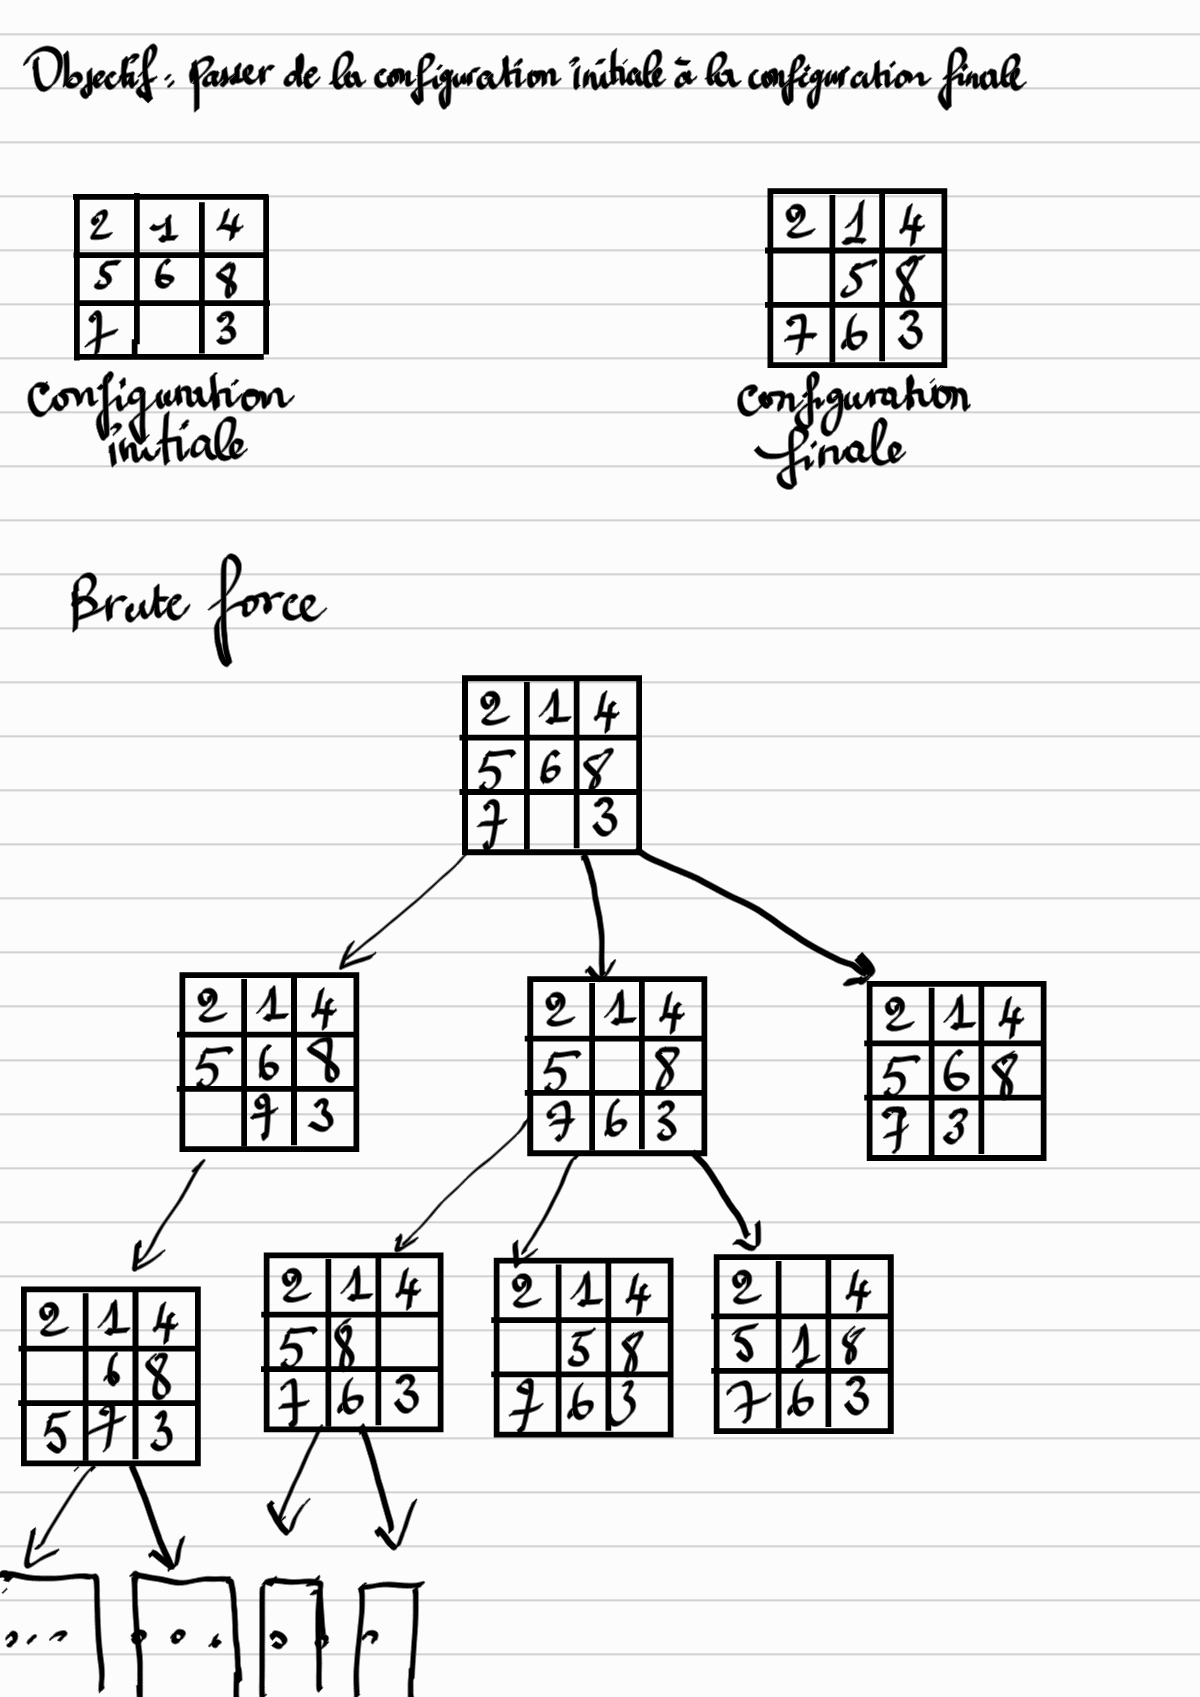
\includegraphics[width=.9\linewidth]{./1.jpg}
\caption{Algorithme bruteforce parcours en profondeur}
\end{figure}



Cependant cette solution a une complexité exponentielle. Donc nous avons plus intérêt à choisir une solution plus efficace qui nous permettra de faire moins de recherche.

Nous allons utiliser le branch and bound pour résoudre cet problème.

Pour débuter, nous allons attribuer des couts à noeuds de l'arbre des possibilités.

Soit c(x) le cout du noeud x. r(x) est le coup permettant d'atteindre le noeud x depuis la racine. s(x) est le coup qui permet d'atteindre la solution.

On a la relation c(x) = r(x) + s(x)

Etablissons les coups suivant :

\begin{itemize}
\item 1 : pour un déplacement dans n'importe quelle direction d'un des numéros vers l'emplacement vide.
\end{itemize}

En considérant cela :
\begin{itemize}
\item r(x) devient la longueur du chemin depuis la racine jusqu'au noeud x.
\item s(x) devient le nombre de sommets dans l'état x qui ne sont pas à leur position dans l'état recherché.
\end{itemize}





\begin{figure}[htbp]
\centering
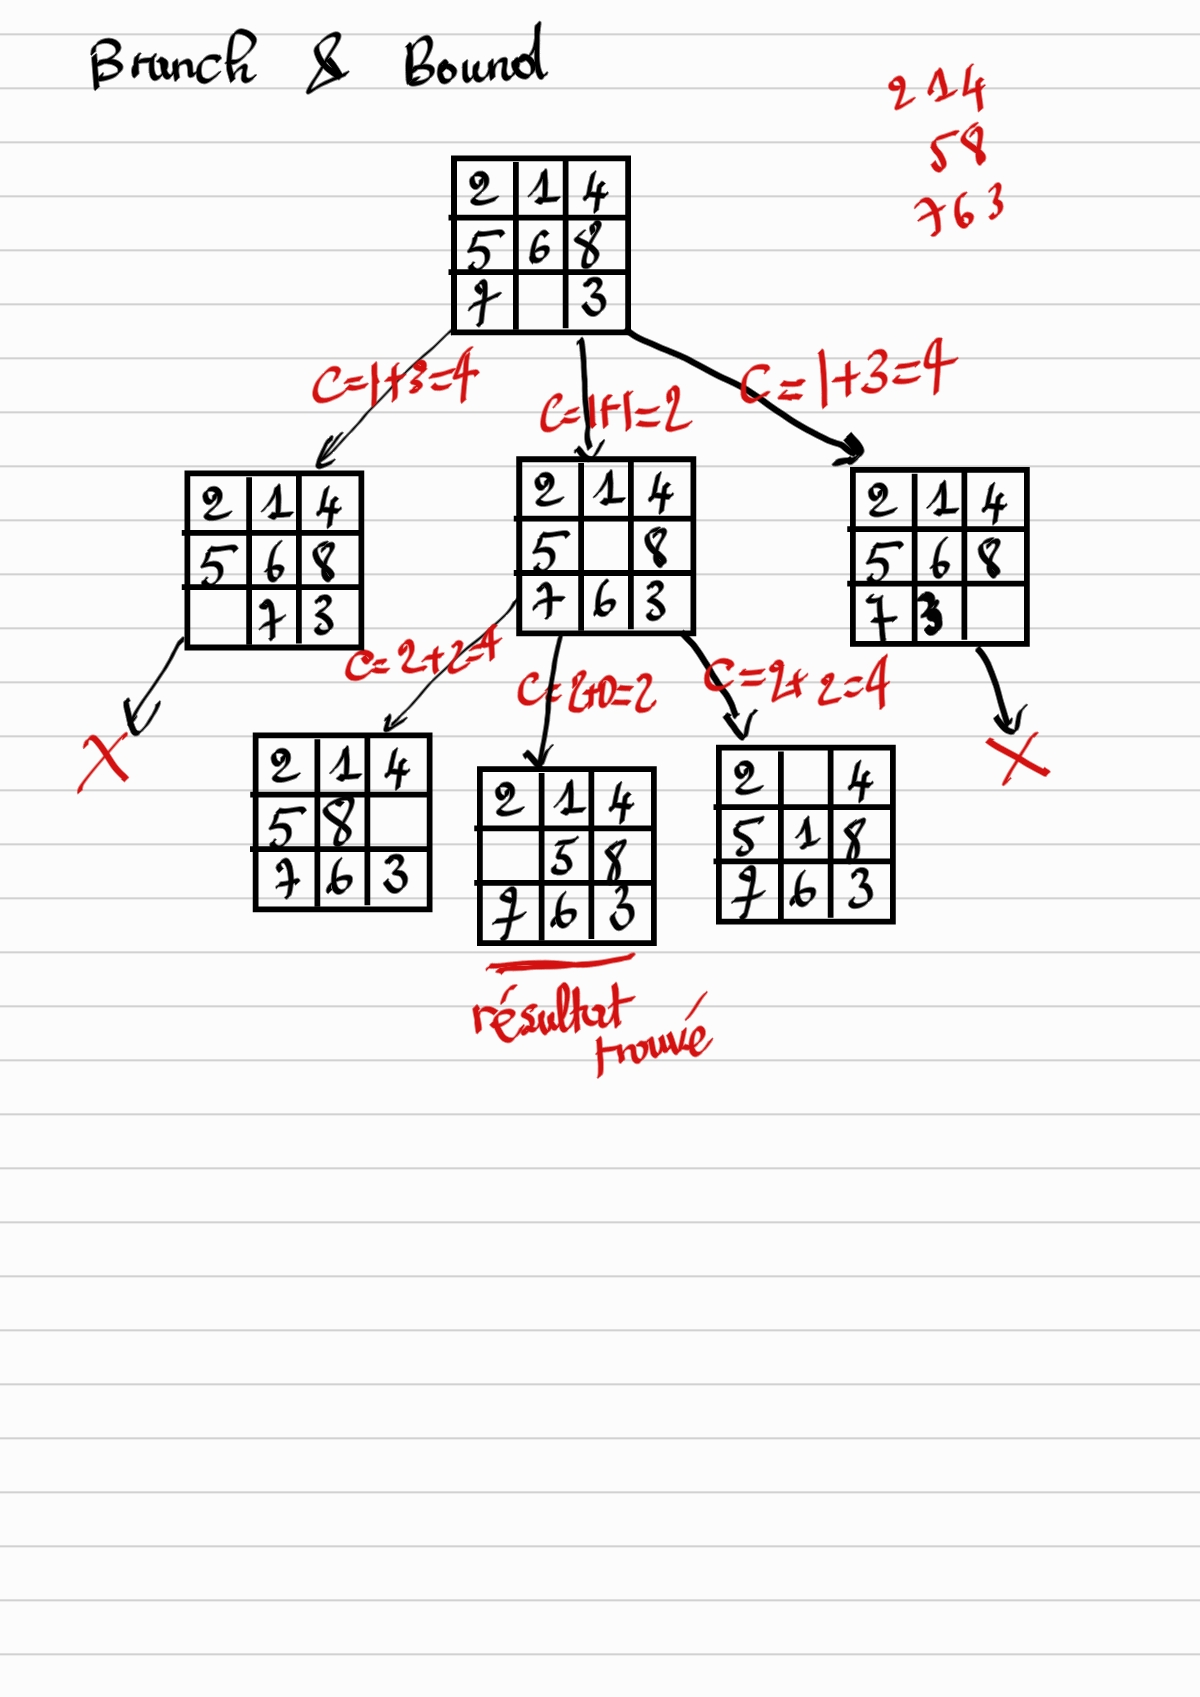
\includegraphics[width=.9\linewidth]{./2.jpg}
\caption{Solution par Branch and Bound}
\end{figure}



\textbf{Programme} (voir annexe)

S'il n'y a pas de solution cet algorithme va tourner à l'infini. Pour résoudre cet problème et afficher le chemin vers la solution la plus proche, il faudrait afficher les chemins en même temps que l'algorithme se déroule, ou plutôt faire la gestion du signal d'arrêt Ctrl+C pour afficher le chemin.



\section{Sources}
\label{sec:org87cee36}

\url{https://chamilo.grenoble-inp.fr/courses/ENSIMAG4MMAOD6/document/resources/index-4MMAOD6.html}


\url{https://www.geeksforgeeks.org}


\url{https://suif.stanford.edu/papers/lam-asplos91.pdf}


\url{https://en.wikipedia.org/wiki/Cache-oblivious\_algorithm\#:\~:text=For\%20example\%2C\%20an\%20optimal\%20cache,in\%20a\%20depth\%2Dfirst\%20fashion}



\clearpage


\section{Annexe}
\label{sec:org70f29f8}


\subsection{illustration principe de localite}
\label{sec:orgcf25544}

\begin{verbatim}
#include <math.h>
#define TAILLE 100

int main(){

    int tab[100] = {0};

    int somme = 0;
    int somme_carres=0;
    for(int i=0; i<sizeof(tab)/sizeof(int); i++){
        somme += tab[i];
    }

    for(int i=0; i<sizeof(tab)/sizeof(int); i++){
        somme_carres += pow(tab[i], 2);
    }
}
\end{verbatim}

\begin{verbatim}
#include <math.h>
#define TAILLE 100

int main(){

    int tab[100] = {0};

    int somme = 0;
    int somme_carres=0;
    for(int i=0; i<sizeof(tab)/sizeof(int); i++){
        somme += tab[i];
        somme_carres += pow(tab[i], 2);
    }

}

\end{verbatim}


\subsection{Optimisation de choix de jeu, programmation dynamique}
\label{sec:orgae0a313}


\emph{strategieJeu.cpp}

\begin{verbatim}
#include <bits/stdc++.h>
using namespace std;

int maxRec(int pieces[], int i, int j, int sum)
{
    if (j == i + 1)
        return max(pieces[i], pieces[j]);

    return max((sum - maxRec(pieces, i + 1, j, sum - pieces[i])),
               (sum - maxRec(pieces, i, j - 1, sum - pieces[j])));
}

int findOptimalStrategy(int* pieces, int n)
{
    int sum = 0;
    sum = accumulate(pieces, pieces + n, sum);
    return maxRec(pieces, 0, n - 1, sum);
}

int main()
{
    int test1[] = { 12, 11, 5, 4 };
    printf("%d\n", findOptimalStrategy(test1, 4));

    int test2[] = { 1, 0, 3, 9 };
    printf("%d\n", findOptimalStrategy(test2, 4));

    int test3[] = { 40, 10, 1, 4, 3, 9 };
    printf("%d\n", findOptimalStrategy(test3, 6));

    return 0;
}
\end{verbatim}


\emph{strategieJeuAvecMemoization.cpp}


\begin{verbatim}
#include <bits/stdc++.h>
using namespace std;

const int N = 100;

int memo[100][100];

int maxRec(int pieces[], int i, int j, int sum)
{
    if (j == i + 1)
        return max(pieces[i], pieces[j]);

    if (memo[i][j] != -1)
        return memo[i][j];


    memo[i][j]
        = max((sum - maxRec(pieces, i + 1, j, sum - pieces[i])),
              (sum - maxRec(pieces, i, j - 1, sum - pieces[j])));

    return memo[i][j];
}


int findOptimalStrategy(int* pieces, int n)
{
    int sum = 0;
    sum = accumulate(pieces, pieces + n, sum);

    memset(memo, -1, sizeof(memo));

    return maxRec(pieces, 0, n - 1, sum);
}

int main()
{
    int test1[] = { 12, 11, 5, 4 };
    printf("%d\n", findOptimalStrategy(test1, 4));

    int test2[] = { 1, 0, 3, 9 };
    printf("%d\n", findOptimalStrategy(test2, 4));

    int test3[] = { 40, 10, 1, 4, 3, 9 };
    printf("%d\n", findOptimalStrategy(test3, 6));

    return 0;
}

\end{verbatim}


\subsection{Branch \& Bound}
\label{sec:org29e1ff3}

\emph{8puzzle.cpp}

\begin{verbatim}
#include <bits/stdc++.h>
using namespace std;
#define N 3

// on considère que le puzzle peut être résolu

class Noeud
{
    public:
    // permet de faire le backtracking
    Noeud* parent;

    // etat actuel du puzzle
    int puzzle[N][N];

    // stores blank tile coordinates
    int x, y;

    // stores the number of misplaced tiles
    int cout;

    // stores the number of moves so far
    int level;
};

// affichage de l'état du puzzle
void printPuzzle(int puzzle[N][N])
{
    for (int i = 0; i < N; i++)
    {
        for (int j = 0; j < N; j++)
            printf("%d ", puzzle[i][j]);
        printf("\n");
    }
}

// Création d'un noeud
Noeud* newNoeud(int puzzle[N][N], int x, int y, int newX,
              int newY, int level, Noeud* parent)
{
    Noeud* noeud = new Noeud;

    noeud->parent = parent;

    memcpy(noeud->puzzle, puzzle, sizeof noeud->puzzle);

    swap(noeud->puzzle[x][y], noeud->puzzle[newX][newY]);

    noeud->cout = INT_MAX;

    noeud->level = level;

    noeud->x = newX;
    noeud->y = newY;

    return noeud;
}

// bottom, left, top, right
int row[] = { 1, 0, -1, 0 };
int col[] = { 0, -1, 0, 1 };

int getCout(int initial[N][N], int final[N][N])
{
    int count = 0;
    for (int i = 0; i < N; i++)
      for (int j = 0; j < N; j++)
        if (initial[i][j] && initial[i][j] != final[i][j])
           count++;
    return count;
}

int isMatrixIndexesOutOfBounds(int x, int y)
{
    return (x >= 0 && x < N && y >= 0 && y < N);
}

void afficherSolution(Noeud* root)
{
    if (root == NULL)
        return;
    afficherSolution(root->parent);
    printPuzzle(root->puzzle);

    printf("\n");
}

struct comp
{
    bool operator()(const Noeud* lhs, const Noeud* rhs) const
    {
        return (lhs->cout + lhs->level) > (rhs->cout + rhs->level);
    }
};

// x et y sont les coordonnées de la case vide
void solve(int initial[N][N], int x, int y,
           int final[N][N])
{
    priority_queue<Noeud*, std::vector<Noeud*>, comp> pq;

    Noeud* root = newNoeud(initial, x, y, x, y, 0, NULL);
    root->cout = getCout(initial, final);

    // Add root to list of live nodes;
    pq.push(root);

    while (!pq.empty())
    {
        Noeud* min = pq.top();

        pq.pop();

        if (min->cout == 0)
        {
            afficherSolution(min);
            return;
        }

        for (int i = 0; i < 4; i++)
        {
            if (isMatrixIndexesOutOfBounds(min->x + row[i], min->y + col[i]))
            {
                Noeud* child = newNoeud(min->puzzle, min->x,
                              min->y, min->x + row[i],
                              min->y + col[i],
                              min->level + 1, min);
                child->cout = getCout(child->puzzle, final);

                pq.push(child);
            }
        }
    }
}

int main()
{
    int initial[N][N] =
    {
        {2, 1, 4},
        {5, 6, 8},
        {7, 0, 3}
    };

    int final[N][N] =
    {
        {2, 1, 4},
        {5, 8, 0},
        {7, 6, 3}
    };

    // L'espace vide se trouve à la position (0, 0)
    int x = 2, y = 1;

    solve(initial, x, y, final);

    return 0;
}

\end{verbatim}
\end{document}